%!TeX program = xelatex
%Do not change
\documentclass[12pt, oneside]{article}
\usepackage{amssymb,amsmath}
\usepackage[margin=1in]{geometry}
\usepackage{textpos}
\usepackage{float}
\usepackage{booktabs}
%\usepackage{color}
\usepackage{graphicx}
\usepackage[inter-unit-product =\cdot]{siunitx}
\let\DeclareUSUnit\DeclareSIUnit
\let\US\SI
\DeclareUSUnit\inch{in}
\DeclareUSUnit\foot{ft}
\DeclareUSUnit\mile{mi}
\DeclareUSUnit\foot{ft}
\DeclareUSUnit\slug{slug}
\DeclareUSUnit\pound{lb}
\DeclareUSUnit\psi{psi}
\DeclareUSUnit\Msi{Msi}
\DeclareUSUnit\ksi{ksi}

\begin{document}

\begin{textblock*}{4cm}(-1.7cm,-2.3cm)
\noindent {\scriptsize AE333 Fall 2021}
\end{textblock*}

%Do not modify other than putting your name where stated
\begin{textblock*}{8cm}(12.5cm,-1cm)
\noindent {Name: }
\end{textblock*}
%Do not modify other than typing your acknowledgement where stated
\begin{textblock*}{13.5cm}(-1.7cm,-1.8cm)
%\noindent \textit{\footnotesize Acknowledgement: Your acknowledgement for collaboration and other sources goes here. }
\end{textblock*}

\vspace{1cm}

%Do not modify other than typing the homework number after #
\begin{center}
\textbf{\Large Homework 7}

\textbf{Due 5 November 2021}
\end{center}

\begin{enumerate}
	\item %8-6
		Find the maximum force, $P$, that can be exerted on the pistons such that the hoop stress in the cylinder does not exceed $\SI{3}{MPa}$.
		Each piston has a radius of $\SI{46}{mm}$ and the cylinder has a wall thickness of $\SI{1 }{mm}$
		\begin{figure}[H]
			\centering
			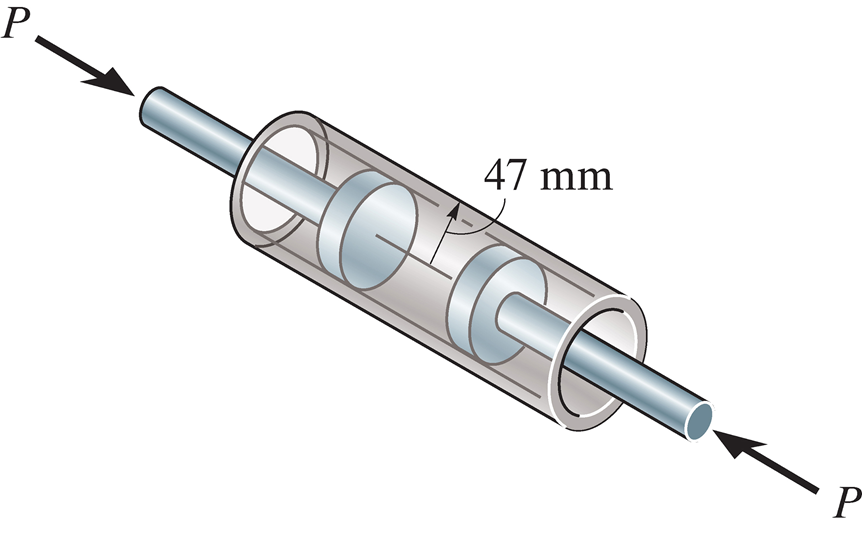
\includegraphics[width=0.6\linewidth]{8-6}
		\end{figure}

	\item %8-9
		The steel water pipe has an inner diameter of $ 	\US{10}{in}  $ and a wall thickness of $ 	\US{.125}{in}  $.
		If the valve at $A$ is closed, find the stresses in the pipe at point $B$ when the water pressure is $ 	\US{250}{psi}  $.
		Sketch the state of stress on a representative element at $B$.
		\begin{figure}[H]
			\centering
			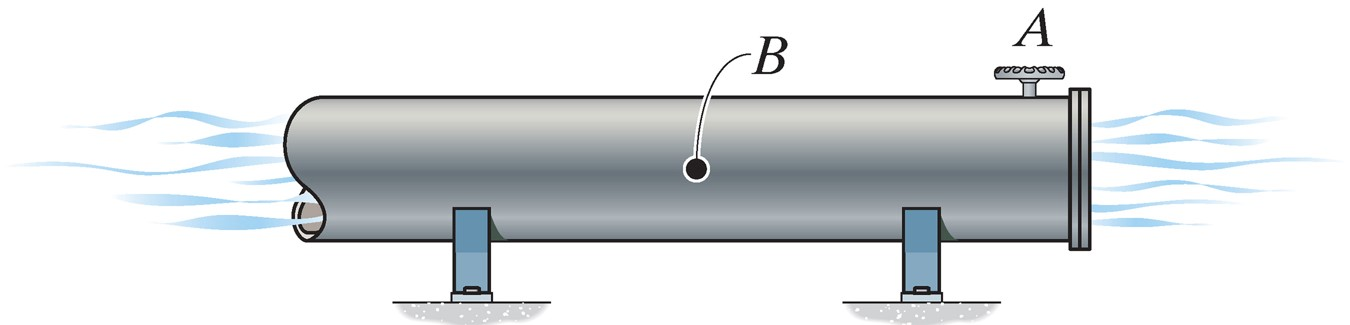
\includegraphics[width=0.6\linewidth]{8-9}
		\end{figure}
		\newpage

	\item %8-27
		The screw of a C-clamp exerts a compressive force of $ 	\US{500}{lb}  $ on the wood blocks.
		Sketch the stress distribution on section $a-a$ of the clamp assuming it has a rectangular cross section of $ 	\US{0.75}{in}  $ tall by $ 	\US{0.25 }{in }  $ thick.
		\begin{figure}[H]
			\centering
			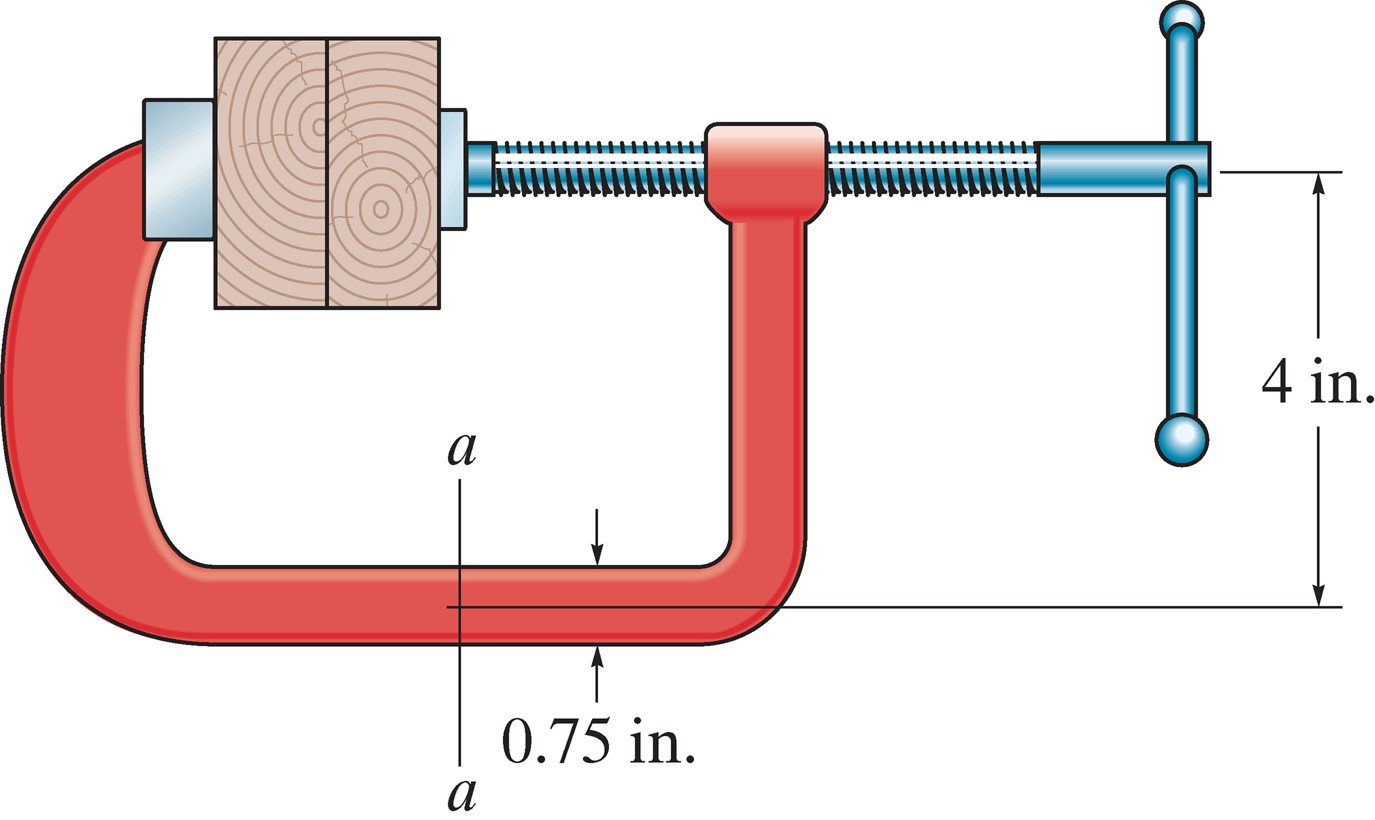
\includegraphics[width=0.6\linewidth]{8-27}
		\end{figure}

	\item %8-52
		The vertebra of the spinal column can support a maximum compressive stress of $\sigma_{max}$ before fracture.
		Find the smallest force, $P$, that would cause fracture if it is applied some distance $e$ away from the centerline of the bone.
		Treat the vertebra as a hollow cylinder.
		\begin{figure}[H]
			\centering
			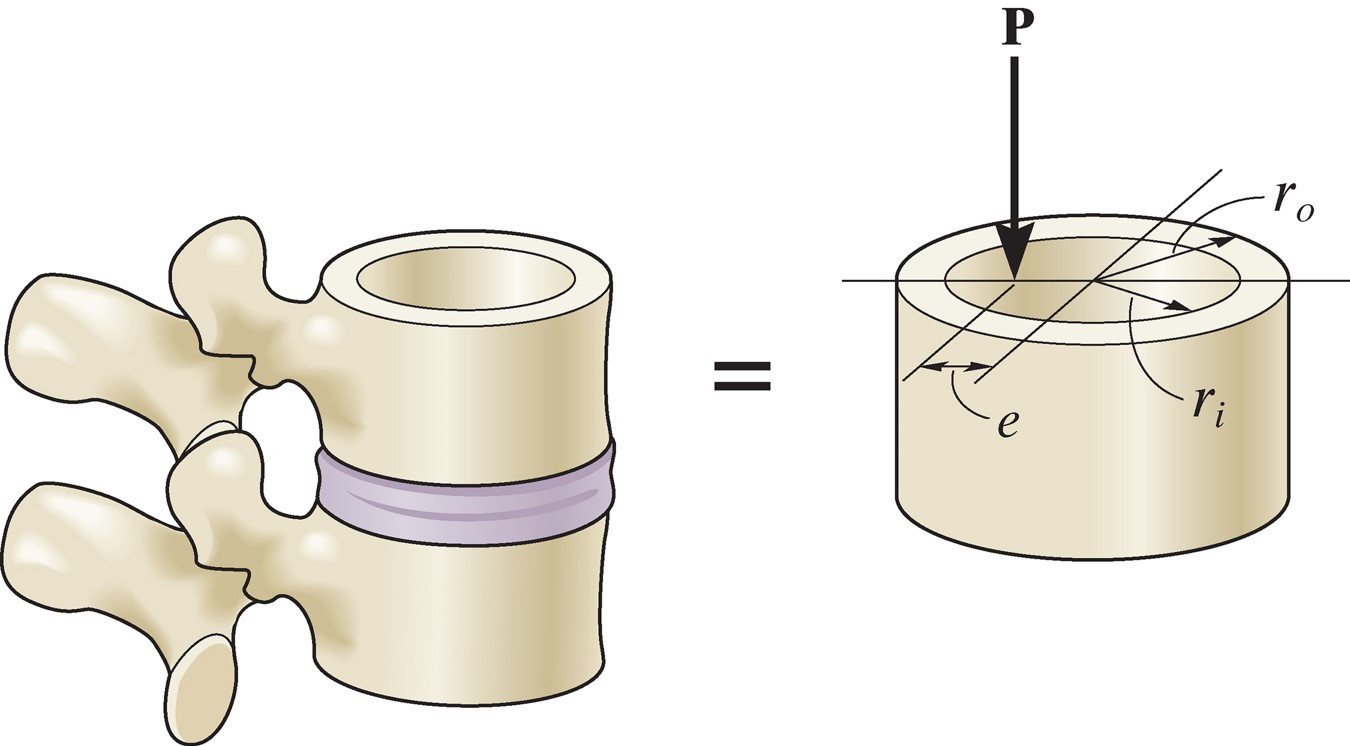
\includegraphics[width=0.6\linewidth]{8-52}
		\end{figure}
		\newpage

	\item %past exam problem?
		Find the state of stress at the point $C$ indicated on the figure.
		\begin{figure}[H]
			\centering
			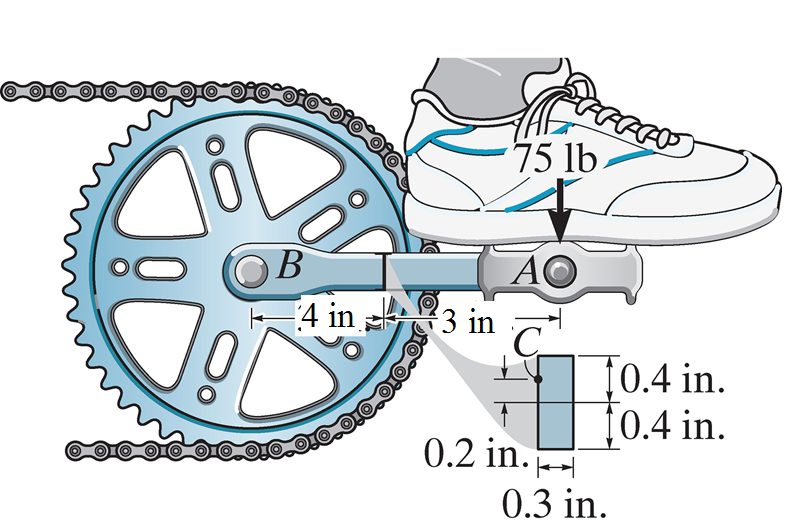
\includegraphics[width=0.6\linewidth]{3-2b}
		\end{figure}

	\item %C8-1
		Explain why this garden hose failed along its length instead of in some other way.
		\begin{figure}[H]
			\centering
			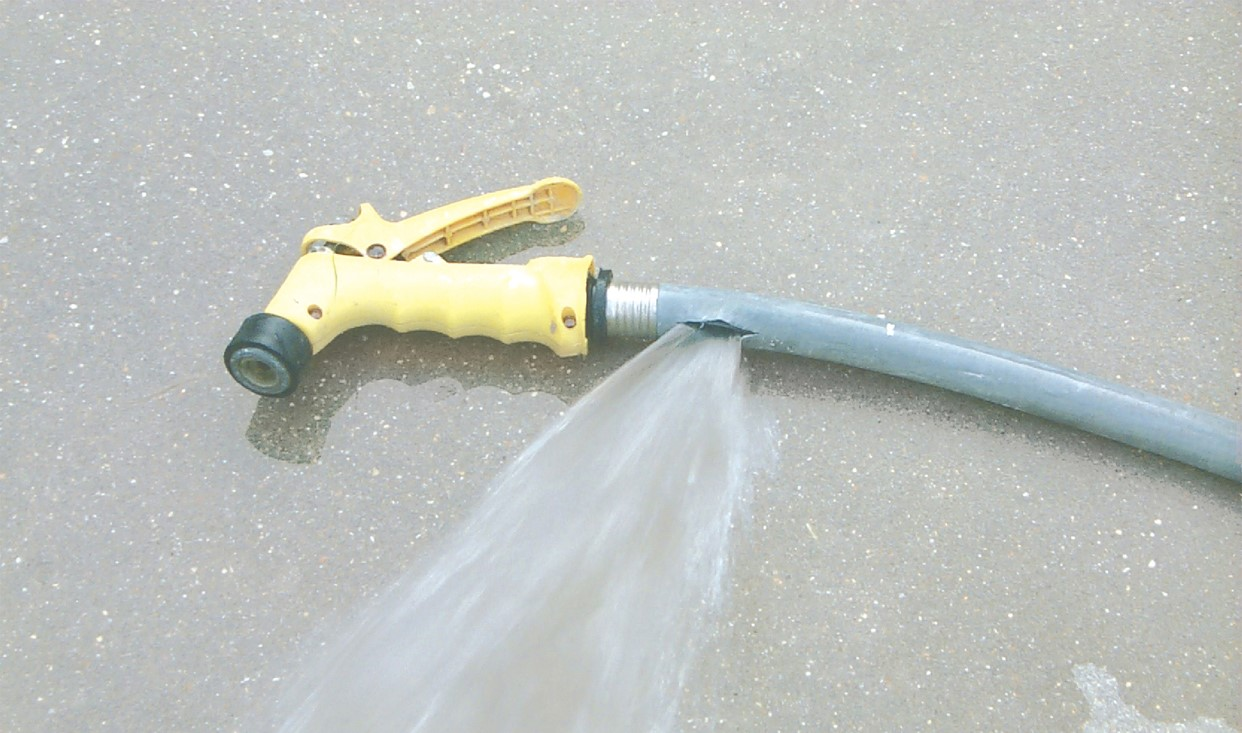
\includegraphics[width=0.6\linewidth]{C8-1}
		\end{figure}
		\newpage

	\item %C8-2
		This open-ended grain silo is used to store wheat or other grain.
		It is built from vertically-oriented wooden slates with steel straps holding them together.
		Explain why the bands are spaced closer together near the bottom compared to the top.
		If each band were to have the same stress, how would you determine the spacing?
		How is this silo different from a thin-walled pressure vessel?
		\begin{figure}[H]
			\centering
			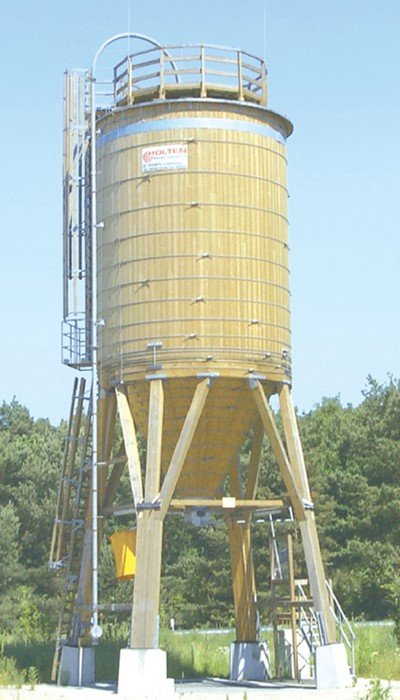
\includegraphics[width=0.6\linewidth]{C8-2}
		\end{figure}

\end{enumerate}
\end{document}
